\documentclass[14pt]{extbook}
\usepackage{multicol, enumerate, enumitem, hyperref, color, soul, setspace, parskip, fancyhdr} %General Packages
\usepackage{amssymb, amsthm, amsmath, bbm, latexsym, units, mathtools} %Math Packages
\everymath{\displaystyle} %All math in Display Style
% Packages with additional options
\usepackage[headsep=0.5cm,headheight=12pt, left=1 in,right= 1 in,top= 1 in,bottom= 1 in]{geometry}
\usepackage[usenames,dvipsnames]{xcolor}
\usepackage{dashrule}  % Package to use the command below to create lines between items
\newcommand{\litem}[1]{\item#1\hspace*{-1cm}\rule{\textwidth}{0.4pt}}
\pagestyle{fancy}
\lhead{Progress Quiz 5}
\chead{}
\rhead{Version C}
\lfoot{9912-2038}
\cfoot{}
\rfoot{Spring 2021}
\begin{document}

\begin{enumerate}
\litem{
Solve the linear equation below. Then, choose the interval that contains the solution.\[ \frac{5x + 4}{8} - \frac{8x -3}{3} = \frac{-5x -8}{7} \]\begin{enumerate}[label=\Alph*.]
\item \( x \in [-1.7, -0.6] \)
\item \( x \in [1.5, 2.4] \)
\item \( x \in [10.9, 12.8] \)
\item \( x \in [0.2, 0.8] \)
\item \( \text{There are no real solutions.} \)

\end{enumerate} }
\litem{
Write the equation of the line in the graph below in Standard form $Ax+By=C$. Then, choose the intervals that contain $A, B, \text{ and } C$.
\begin{center}
    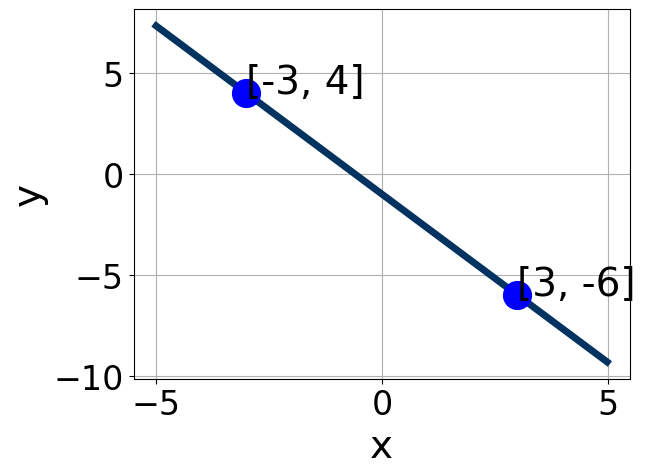
\includegraphics[width=0.5\textwidth]{../Figures/linearGraphToStandardC.png}
\end{center}
\begin{enumerate}[label=\Alph*.]
\item \( A \in [0, 2.2], \hspace{3mm} B \in [0.94, 2.57], \text{ and } \hspace{3mm} C \in [-1.2, -0.8] \)
\item \( A \in [2.5, 5.2], \hspace{3mm} B \in [-3.82, -2.9], \text{ and } \hspace{3mm} C \in [2.3, 5] \)
\item \( A \in [2.5, 5.2], \hspace{3mm} B \in [2.07, 3.41], \text{ and } \hspace{3mm} C \in [-6.6, -2] \)
\item \( A \in [-6.9, -2.9], \hspace{3mm} B \in [-3.82, -2.9], \text{ and } \hspace{3mm} C \in [2.3, 5] \)
\item \( A \in [0, 2.2], \hspace{3mm} B \in [-1.51, -0.08], \text{ and } \hspace{3mm} C \in [-0.8, 1.3] \)

\end{enumerate} }
\litem{
Solve the equation below. Then, choose the interval that contains the solution.\[ -6(-16x -9) = -4(10x -11) \]\begin{enumerate}[label=\Alph*.]
\item \( x \in [-1.9, -1.1] \)
\item \( x \in [0.6, 1.5] \)
\item \( x \in [-0.3, 0.2] \)
\item \( x \in [-1.7, -0.3] \)
\item \( \text{There are no real solutions.} \)

\end{enumerate} }
\litem{
First, find the equation of the line containing the two points below. Then, write the equation as $ y=mx+b $ and choose the intervals that contain $m$ and $b$.\[ (-10, 2) \text{ and } (6, -9) \]\begin{enumerate}[label=\Alph*.]
\item \( m \in [-1.44, 0.13] \hspace*{3mm} b \in [-16.3, -13.7] \)
\item \( m \in [-1.44, 0.13] \hspace*{3mm} b \in [9.9, 15.6] \)
\item \( m \in [-1.44, 0.13] \hspace*{3mm} b \in [-6.9, -3] \)
\item \( m \in [-0.56, 1.01] \hspace*{3mm} b \in [-14.5, -10.5] \)
\item \( m \in [-1.44, 0.13] \hspace*{3mm} b \in [1.6, 7] \)

\end{enumerate} }
\litem{
First, find the equation of the line containing the two points below. Then, write the equation as $ y=mx+b $ and choose the intervals that contain $m$ and $b$.\[ (-4, 6) \text{ and } (-2, 3) \]\begin{enumerate}[label=\Alph*.]
\item \( m \in [-0.5, 2.6] \hspace*{3mm} b \in [5.85, 7.27] \)
\item \( m \in [-4.1, 0.5] \hspace*{3mm} b \in [-1.47, 0.3] \)
\item \( m \in [-4.1, 0.5] \hspace*{3mm} b \in [4.78, 5.84] \)
\item \( m \in [-4.1, 0.5] \hspace*{3mm} b \in [-1.47, 0.3] \)
\item \( m \in [-4.1, 0.5] \hspace*{3mm} b \in [9.92, 11.12] \)

\end{enumerate} }
\litem{
Write the equation of the line in the graph below in Standard form $Ax+By=C$. Then, choose the intervals that contain $A, B, \text{ and } C$.
\begin{center}
    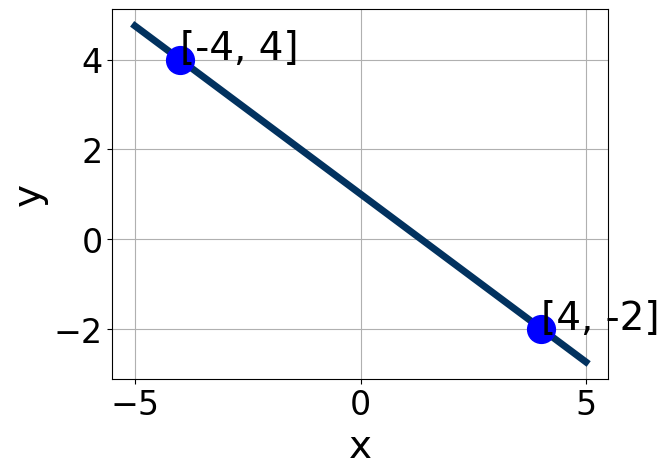
\includegraphics[width=0.5\textwidth]{../Figures/linearGraphToStandardCopyC.png}
\end{center}
\begin{enumerate}[label=\Alph*.]
\item \( A \in [1.6, 5.3], \hspace{3mm} B \in [-5.22, -3.84], \text{ and } \hspace{3mm} C \in [-5.79, -3.85] \)
\item \( A \in [-1, 2.2], \hspace{3mm} B \in [-3.39, 0.19], \text{ and } \hspace{3mm} C \in [-1.89, -0.73] \)
\item \( A \in [1.6, 5.3], \hspace{3mm} B \in [2.54, 4.5], \text{ and } \hspace{3mm} C \in [3.4, 4.08] \)
\item \( A \in [-3.5, -2.7], \hspace{3mm} B \in [-5.22, -3.84], \text{ and } \hspace{3mm} C \in [-5.79, -3.85] \)
\item \( A \in [-1, 2.2], \hspace{3mm} B \in [0.29, 1.96], \text{ and } \hspace{3mm} C \in [0.72, 1.37] \)

\end{enumerate} }
\litem{
Solve the equation below. Then, choose the interval that contains the solution.\[ -16(-10x -4) = -13(-17x -6) \]\begin{enumerate}[label=\Alph*.]
\item \( x \in [2.03, 2.39] \)
\item \( x \in [-2.91, -1.84] \)
\item \( x \in [-0.96, -0.37] \)
\item \( x \in [-0.28, 0.4] \)
\item \( \text{There are no real solutions.} \)

\end{enumerate} }
\litem{
Find the equation of the line described below. Write the linear equation as $ y=mx+b $ and choose the intervals that contain $m$ and $b$.\[ \text{Parallel to } 7 x + 3 y = 3 \text{ and passing through the point } (-3, 2). \]\begin{enumerate}[label=\Alph*.]
\item \( m \in [-3.33, -1.33] \hspace*{3mm} b \in [1, 7] \)
\item \( m \in [-0.43, 1.57] \hspace*{3mm} b \in [-5, 1] \)
\item \( m \in [-3.33, -1.33] \hspace*{3mm} b \in [-5, 1] \)
\item \( m \in [2.33, 7.33] \hspace*{3mm} b \in [6, 11] \)
\item \( m \in [-3.33, -1.33] \hspace*{3mm} b \in [1, 7] \)

\end{enumerate} }
\litem{
Solve the linear equation below. Then, choose the interval that contains the solution.\[ \frac{-4x + 6}{3} - \frac{-7x -9}{2} = \frac{-4x + 5}{7} \]\begin{enumerate}[label=\Alph*.]
\item \( x \in [1, 2] \)
\item \( x \in [-4.5, -2.8] \)
\item \( x \in [-1.9, -0.8] \)
\item \( x \in [-2.6, -1.8] \)
\item \( \text{There are no real solutions.} \)

\end{enumerate} }
\litem{
Find the equation of the line described below. Write the linear equation as $ y=mx+b $ and choose the intervals that contain $m$ and $b$.\[ \text{Parallel to } 3 x - 5 y = 7 \text{ and passing through the point } (6, 5). \]\begin{enumerate}[label=\Alph*.]
\item \( m \in [-1.42, -0.58] \hspace*{3mm} b \in [8.53, 9.81] \)
\item \( m \in [0.54, 0.75] \hspace*{3mm} b \in [1.16, 2.09] \)
\item \( m \in [0.54, 0.75] \hspace*{3mm} b \in [-1.14, -0.76] \)
\item \( m \in [0.54, 0.75] \hspace*{3mm} b \in [-1.67, -1.11] \)
\item \( m \in [1.08, 2.03] \hspace*{3mm} b \in [1.16, 2.09] \)

\end{enumerate} }
\end{enumerate}

\end{document}